% Roll Number 31, Harikrishnan G

\textbf{\textcolor{LightMagenta}{Explain the concept of Overfitting and Underfitting model with suitable diagrams. (Dec 2019) \hfill 4 marks}} \\[5pt]
When we are working on a data set for predicting or classifying, we calculate accuracy for our model. If the accuracy is low or average, we tends to increase the accuracy by increasing or decreasing data features in our model. Sometimes, this creates our model to perform poorly. It is because of either the model is too simple to describe the data \textbf{(underfitting)}, or too complex in describing the data \textbf{(overfitting)}.\\
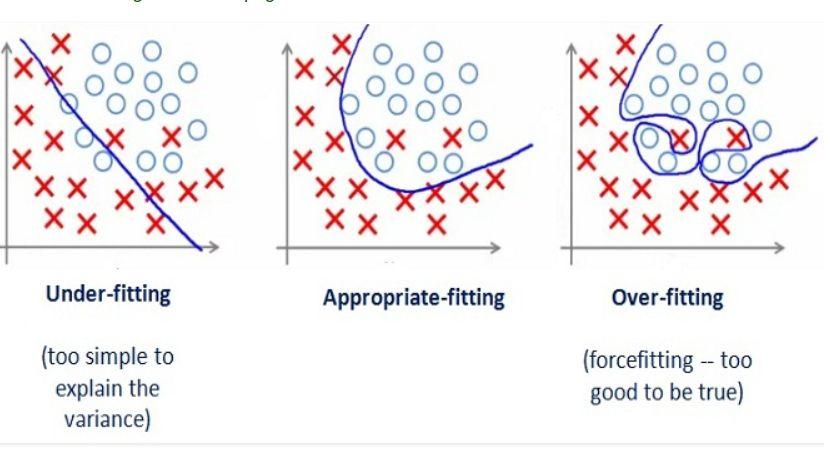
\includegraphics[scale=0.65]{Images/A36_img2.jpg}
\begin{itemize}
    \item When we look at the left graph, it does not cover all points in the graph. Such model gives poor results due to underfitting of the data, which is also called High Bias. 
    \item When we look at the right graph, it covers each and every point in the graph. We might think that it is a very good model, but it is not because it covers all noises and outliers in the data provided. Such model also gives poor results due to overfitting of the data, which is also called High Variance. 
    \item Now look at the middle graph. It covers all important points and leaves out noises and outliers. Hence it gives the best results.
    \item Bias means how much we ignore the data, so high bias means we ignore too much data. Variance means how much we are dependent on the data, so high variance means we are too much dependent/reliant on the data. In any model, there will be trade off between bias and variance. But we try to achieve the best balance.
    \item Though underfitting and overfitting leads to poor performance, common problem of these two is overfitting. To limit overfitting, two techniques are used:
    \begin{itemize}
        \item Validation
        \item K-fold Cross-Validation
    \end{itemize}
\end{itemize} \\